\documentclass[12pt]{article}

\addtolength{\textwidth}{.8in}
\addtolength{\hoffset}{-.4in}
\addtolength{\textheight}{1in}
\addtolength{\voffset}{-1in}

\usepackage{amsmath}
\usepackage{graphicx}
\usepackage{upquote} % to convert funny quotes to straight quotes
\usepackage{amsfonts}
\usepackage{paralist}
\setlength{\parindent}{15pt}

\renewcommand*{\thefootnote}{\fnsymbol{footnote}}

% what a log is
% identities (turn multiplicative things into additive things)
%     log(xy) = log(x) + log(y)
%     log(x^a) = a log(x)
% semi-log and log-log plots.
%  How to do in Python (.xscale(), .yscale())
%  Three reasons they're useful:
%    - rein in large variations of the data
%          rein.py example
%          New Zealand example (archive.stats.govt.nz/infoshare,
%              Tourism > International Travel and Migration > Visitor 
%                  Arrival Totals (Monthly)
%                  (see nz.py and nz.csv in teaching/219)
%    - show multiplicative changes:
%          stock.py example
%    - reveal exp & power-law behavior
%        - derive why
%          logplots.py example -- show power law & exp -> straight lines
% exponential vs. power-law; "fat tails" "scale-free"
%     exp_vs_power.py
%     expected value of exp, and power-law...doesn't exist!
% animal example

\begin{document}

\begin{center}
\begin{Large}
DATA 219 Notes -- Mar. 1, 2018
\end{Large}
\end{center}

\section{Review of logarithms}

Recall that the logarithm is the inverse operation of exponentiation. What is
$10^3$? 1,000. So what is the log of 1,000? 3. It's really that simple.
Instead of asking, ``what is ten to this particular power?" I'm asking ``what
power would I raise 10 to in order to get this particular number?"

(This is assuming we're using ``base-10 logarithms," notated as
$\log_{10}$. You can use any other base as well: common choices are 
2 (sometimes $\log_{2}$ is abbreviated ``$\lg$"),
$e$ ($\log_{e}$, the ``natural" logarithm, is usually abbreviated ``$\ln$"),
and 10 ($\log_{10}$ is often just plain ``$\log$".))

The role of the logarithm is to mercilessly crush numbers down to size.

\begin{center}
\begin{tabular}{c|c}
$x$ & $\log x$ \\
\hline
1 & 0 \\
10 & 1 \\
100 & 2 \\
1,000 & 3 \\
10,000 & 4 \\
100,000 & 5 \\
... & ... \\
\end{tabular}
\end{center}

Enormous numbers -- in the millions -- get squished down to single digits, and
\textit{the squashing gets more dramatic as the size of the number grows}.
Jumping from 1 to 10 (a difference of 9) netted us one higher in terms of
logarithm, but jumping from 10 all the way to 100 (a difference of
\textit{90}) \textit{also} only got us one higher. It's this property that
makes logarithms useful.

Another way to think of logarithms is ``the logarithm of $x$ is the order of
magnitude of $x$."

One property of logarithms that is extremely important to know is this:
\begin{align*}
\log(xy) = \log(x) + \log(y)
\end{align*}
Thus logarithms effectively \textit{turn multiplications into additions}. One
practical implication of this truth is leveraged in natural language
processing systems: we often find ourselves multiplying minuscule quantities
(very close to zero) and as we multiply these, we get closer and closer to
zero to the point where Python doesn't have enough precision to calculate a
precise number that low. But by dealing with logarithms, we're adding instead
of multiplying and avoid that problem completely.

A natural consequence of the above property is this one:
\begin{align*}
\log(x^a) = a \log(x)
\end{align*}

\section{Logarithmic plots}

A common plotting technique is to use not the raw values of the independent
variable on the $x$ axis, but rather their logarithms. If we do this, we have
a \textbf{semilog plot}. If we do this for both the $x$ and the $y$ axis, we
have a \textbf{log-log plot}.

Why would we do this? There are three reasons:
\begin{enumerate}
\itemsep.1em
\item It reins in large variations in the data. If some of our data points are
orders of magnitude larger than others, the detail of the smaller points gets
completely swamped in trying to plot the larger points. Plotting
orders-of-magnitude instead of raw values solves this problem, though you have
to remember you did this when interpreting the plot!

Here's a (fictitious) example of some American and British celebrities, and
their total Instagram ``likes":
\footnotesize
\begin{Verbatim}[fontsize=\small,samepage=true,frame=none]
plt.plot(uk, linestyle='None', color="red", marker=".", label="UK")
plt.plot(us, linestyle='None', color="green", marker=".", label="US")
plt.yscale('log')
plt.legend()
plt.show()
\end{Verbatim}
\normalsize
\begin{center}
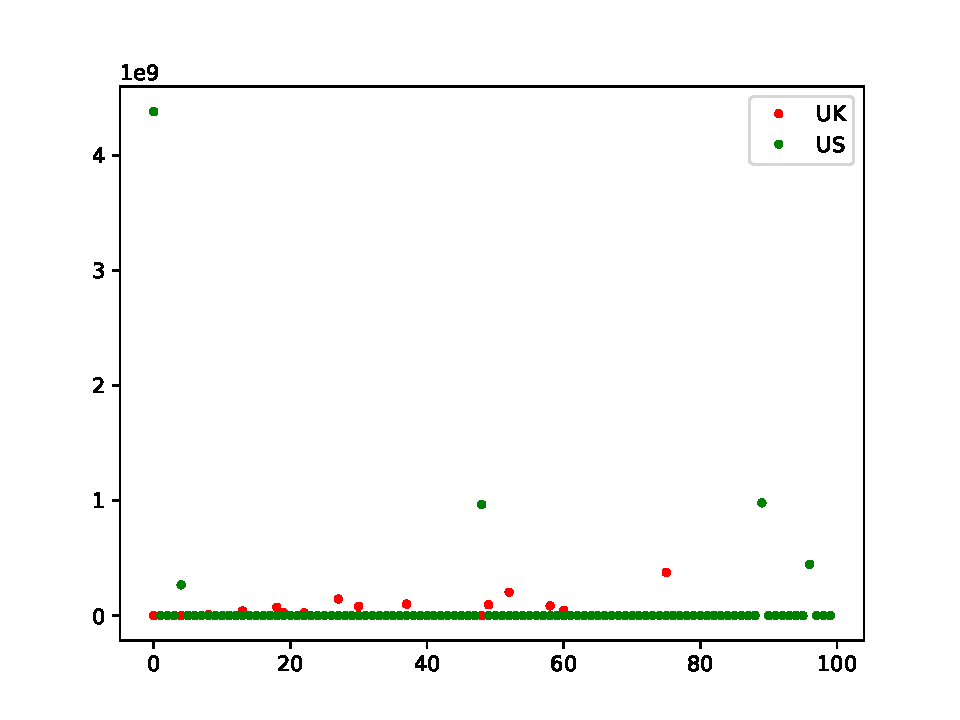
\includegraphics[width=0.7\textwidth]{rein1.pdf}
\end{center}

This plot has limited use, because there are a few uber-celebrities (Justin
Bieber, \textit{etc.}) who have far more ``likes" than anyone else. Hence
most people are crushed against the bottom of the plot and we can't (say)
compare the UK people with the US people easily.

We can dramatically improve the readability and analyze-ability by plotting
the $y$ axis on a log scale. Just add this line before \texttt{plt.show()}:
\begin{Verbatim}[fontsize=\small,samepage=true,frame=none]
plt.yscale('log')
\end{Verbatim}

and voila:

\begin{center}
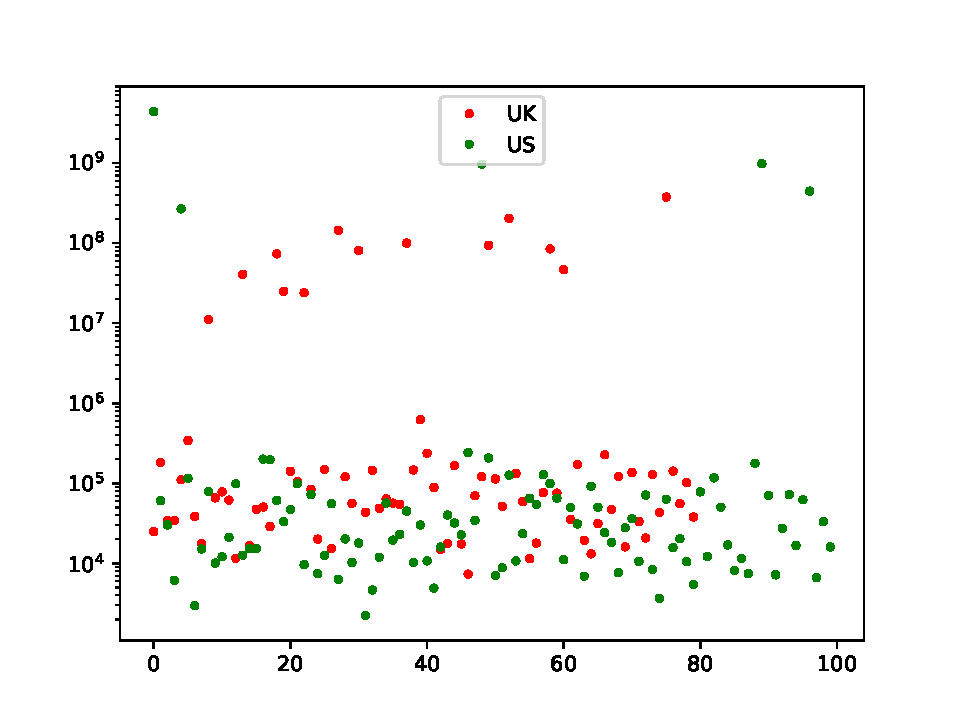
\includegraphics[width=0.7\textwidth]{rein2.pdf}
\end{center}

It's imperative that when you do this, you remember that the $y$-axis no
longer represents number-of-likes, but log-number-of-likes.

\item A semi-log plot shows relative (multiplicative) changes instead of
absolute (additive) changes. Consider this (ordinary linear, not semi-log)
plot of a fictional company's stock price over time:
\begin{center}
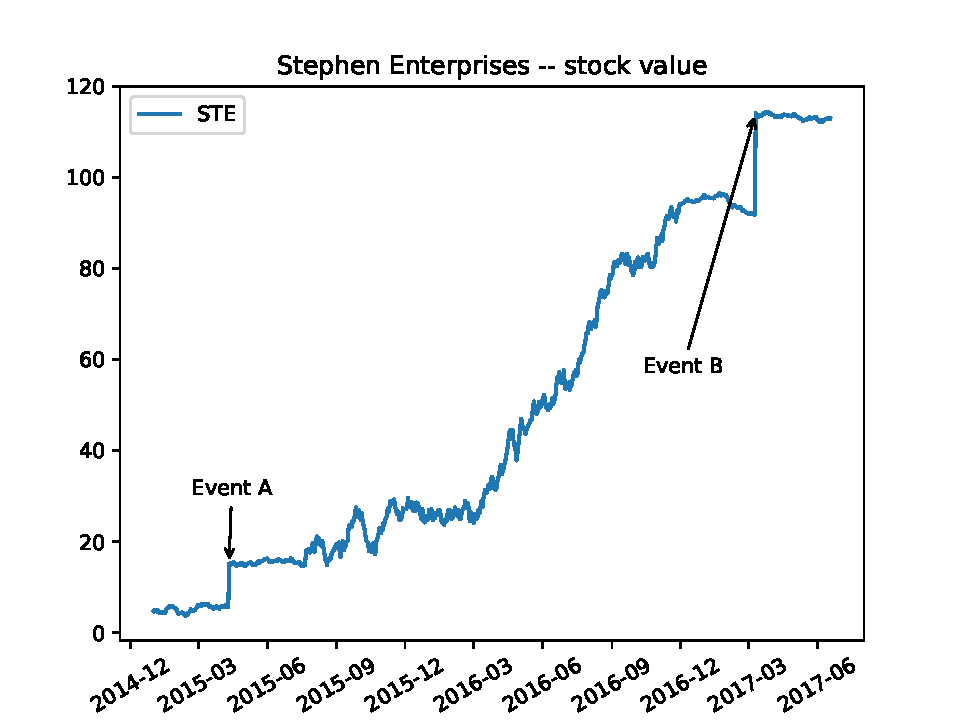
\includegraphics[width=0.8\textwidth]{stock1.pdf}
\end{center}

Two significant events occurred in this company's history: one in April 2015
and the other in March 2017. Both caused the stock's value to jump. Question:
would you rather have bought stock immediately before event A and sold it
immediately after, or done the same before/after B?

On this linear plot, it may look like event B is the better bet: after all, it
looks like the jump was higher. But this is an \textit{absolute} distance: in
other words, the total number of dollars per share jumped higher for event B.
But for something like an investment, you actually don't care about this
absolute number, but the \textit{relative} number. 

Look carefully at event A: before the jump, the stock was selling at about \$5
per share, and afterwards, at about \$15. This means that if you timed this
right, you \textit{tripled your money}! (Buy \$1000 worth of stock in April
2015, and you sell it for \$3000 the following day.) Compared to event B, this
is a way better deal. Consider that at event B, the stock went from \$90 to
\$110. Sure, \$20 is more than \$10 in absolute dollar terms, but if you
bought \$1000 worth of stock in March 2017 and sold it the following day,
you'd have sold it for \$$1000 \times \frac{110}{90} = $\$1222. Nice, but not
nearly the windfall of event A.

For this reason, stocks and other investments are nearly always shown on a
semi-log plot, like so:
\begin{center}
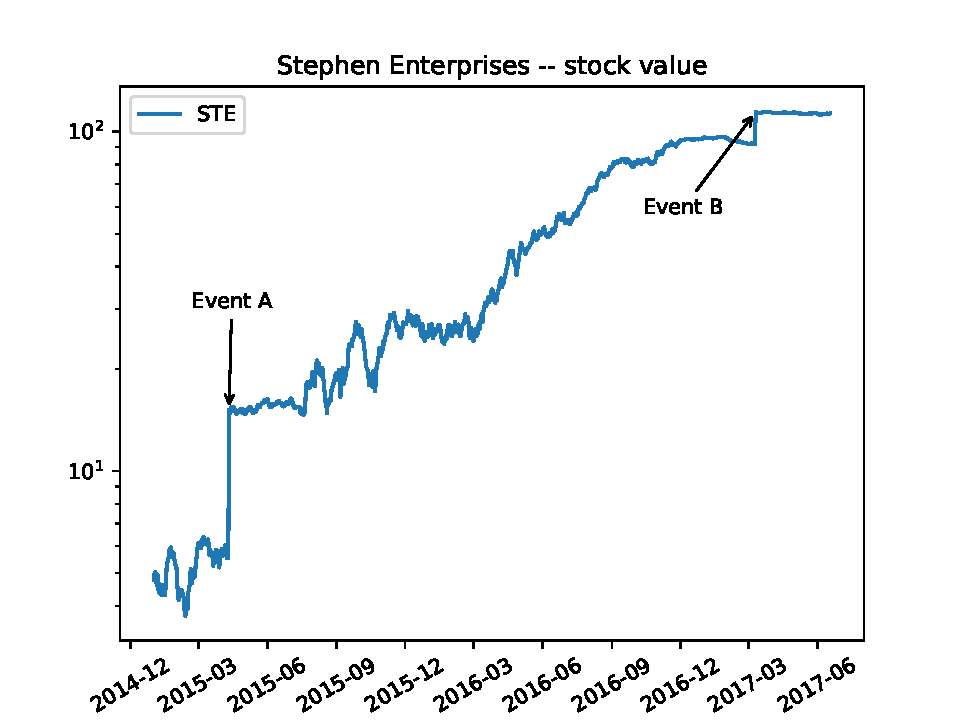
\includegraphics[width=0.8\textwidth]{stock2.pdf}
\end{center}

This has the advantage that \textit{same-size increases on the (log) $y$ axis
correspond to identical \textit{relative} (multiplicative) increases of the
stock.} In other words, if the stock rises an inch somewhere on the plot, and
it rises an inch somewhere else, these represent equal gains for investors
\textit{no matter how high the stock value is in absolute terms.} Such is the
magic of logs.

In this example, you can easily see from the semi-log plot that event A was a
bigger windfall for investors than event B.

\item They reveal exponential and power-law relationships. This requires a
little math to understand. Suppose we have two variables, $x$ and $y$, and
they are related according to something like this:
\begin{align*}
y = p \cdot e^{qx}
\end{align*}
where $p$ and $q$ are just numbers. For example,
\begin{align*}
y = 5.2 \cdot e^{2.96 x}
\end{align*}
Now if we plot $x$ vs $y$ on a standard plot, we get a curvy exponential
function that is very difficult for the human eye to distinguish from other
curvy functions. But suppose we plot not $y$, but $\log y$? Using our
properties from above, we get:
\small
\begin{align*}
\ln y &= \ln (5.2 \cdot e^{2.96 x}) \\
&= \ln(5.2) + \ln(e^{2.96 x}) \\
&= 1.649 + 2.96 x \\
\end{align*}
This is just a linear equation with a slope ($m$) of 2.96 and a $y$-intercept
($b$) of 1.649. So plotting this relationship on a semi-log plot will give us
a straight line.

Why do we care? Because it turns out that exponential relationships like this
come up a lot in the world. One ubiquitous pattern is that of exponential
growth or decay: any time that \textit{the rate of increase of a quantity}
(like the number of new baby rabbits added to a rabbit population) is
proportional to \textit{the quantity itself} (the number of existing rabbits),
we have exponential growth. And any time that the rate of \textit{de}crease of
a quantity (like the number of mechanical parts that wear out) is proportional
to the quantity itself (the number of machines we own), we have exponential
decay.

Another important kind of relationship is often mistaken for exponential
growth, but is emphatically \textit{not}. It's called a ``power-law"
relationship, and has caused much buzz in the scientific community over the
past decade or so. It occurs when we have a simple polynomial relationship:
\begin{align*}
y = p \cdot x^{q}
\end{align*}
where $p$ and $q$ are just numbers. For example,
\begin{align*}
y = 3.9 \cdot x^{-2.45}
\end{align*}

Again, some math: if we take the logarithm of both sides, we get:
\small
\begin{align*}
\ln y &= \ln (3.9 \cdot x^{-2.45}) \\
\ln y &= \ln (3.9) + \ln (x^{-2.45}) \\
\ln y &= 1.361 -2.45 \ln (x) \\
\end{align*}
\normalsize

\vspace{-.25in}
If we plot not $y$ vs $x$, but $\ln y$ vs $\ln x$ (in other words, a
\textbf{log-log plot}, we will get a straight line. (You can see this by
mentally substituting your letter of choice for $\ln x$ and another letter of
your choice for $\ln y$. Now you have a plain old linear equation with a slope
of -2.45 and an intercept of 1.361.)

To see how the logarithmic plots reveal this, consider the following synthetic
data set, where the blue points are linear in $x$, the red points are
exponential, and the green points are power-law (with an exponent of 6):

\begin{center}
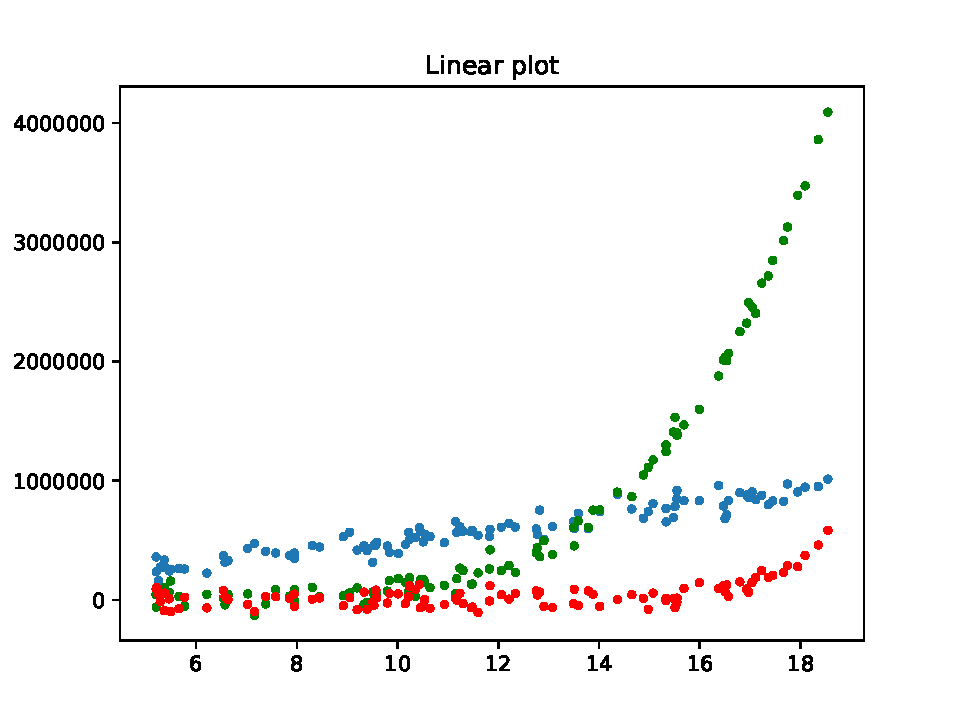
\includegraphics[width=0.3\textwidth]{logplots1.pdf}
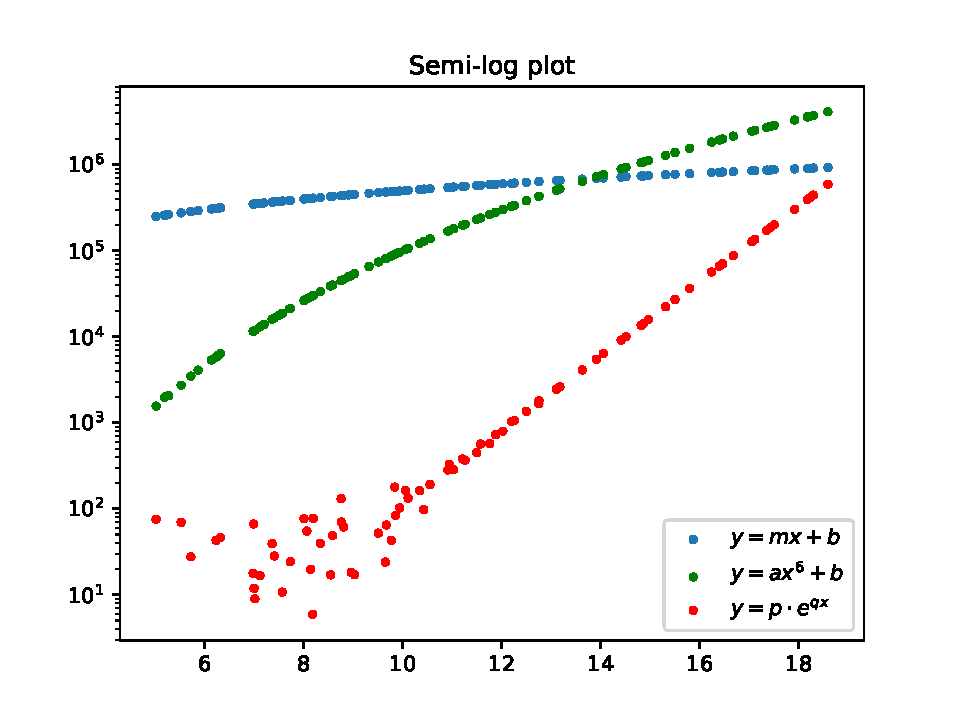
\includegraphics[width=0.3\textwidth]{logplots2.pdf}
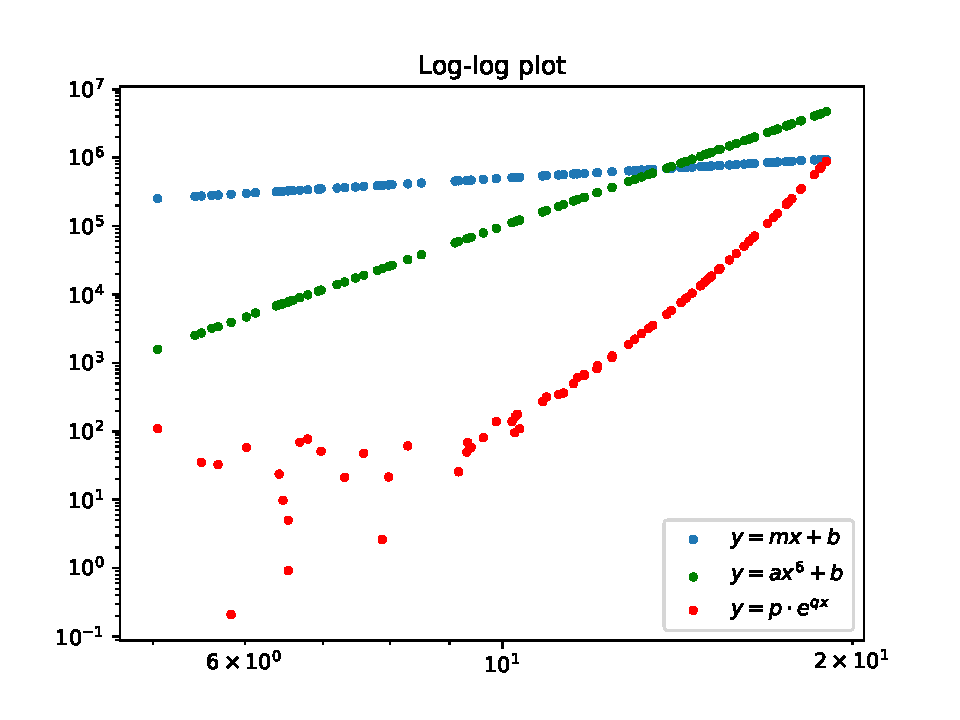
\includegraphics[width=0.3\textwidth]{logplots3.pdf}
\end{center}

In the linear plot, the blue points can be seen to be a straight line. In the
semi-log plot, the red points are. In the log-log plot, the green points are.
This is a powerful tool for recognizing these important kinds of relationships
at a glance.
\end{enumerate}
\end{document}
